%
% Draft  document diamlen.tex
% Questions regarding control of fibre diameter and length growth rate
%
 
\documentclass[titlepage]{article}  % Latex2e
\usepackage{graphicx,lscape,subfigure}
\usepackage{bm}
\usepackage{textcomp}
 

\title{Questions regarding developmental control of fibre diameter and fibre length growth rate in sheep}
\author{Neville Jackson and  Paul Swan}
\date{19 Sep 2018} 

 
\begin{document} 
 
\maketitle      
\tableofcontents

\clearpage
\section{Introduction} 
This is not a research paper or a review. What we are trying to do is set down some ideas relevant to control of fibre diameter and fibre length growth rate in sheep. 

The focus is on fibre diameter. We know that the number of papilla cells in a follicle bulb partly determines the diameter of the fibre grown. We want to  underatand what else is involved so that we can understand how variation in fibre diameter between and along fibres arises. 

Fibre length growth rate is included, because it is felt that understanding the relationship between diameter and length will help to unravel the diameter control issue. 

\section{The papilla cell model}
The fleece of a Merino sheep consists of something of the order of 100 million wool follicles each growing a fibre of approximate circular cross section whose diameter may be anything from 10 to 50 microns, and may vary along the  length of the fibre. The length growth rate of individual fibres may be between 100 and 1000 microns per day. 

The determination of follicle number is understood. The work of Moore and Jackson(1984)~\cite{moor:84}, Moore, Jackson and Lax(1989)~\cite{moor:89}, and Moore, Jackson, Isaacs, and Brown (1998)~\cite{moor:98} suggests that a population of cells known as pre-papilla cells is responsible for follicle initiation at sites at which these cells aggregate. These pre-papilla cells end up in the papilla cavity of the follicle bulb, and the number of papilla cells in a bulb tend to relate to the size of the follicle and the diameter of the fibre it grows.

We can calculate the consequences for follicle number from assuming various combinations of parameters of the papilla cell population and its dynamics and differentiation. There is a writeup and software for this calculation (Jackson and Moore (2018)~\cite{jack:18}). There is also a writeup (Swan(1999)~\cite{swan:99}) which tackles the algebra of pre-papilla cell population numbers. If we assume a relation between papila cell number and fibre diameter, we can even calculate mean fibre diameters.

We do have an empirical relationship between average no of papilla cells per follicle and mean fibre diameter. It is in Figure 4 of Jackson and Moore (2018)~\cite{jack:18}. The correlation in Figure 4 is 0.81 - so only 67 percent of the variance in papilla cell number is explained by fibre diameter. There is room for some other effects to operate. Figure 4 is a mix of sheep from four selection lines. There is no evidence that any selection line deviates from the linear regression line.

However there is more to fibre diameter variation than the number of papilla cells can explain. Mean fibre diameter is a character with an enormous amount of phenotypic plasticity - it varies with seasonal conditions resulting in variation in diameter along the fibre. Papilla cells may be involved in controlling this variation. In species which undergo a regular hair growth cycle, papilla cells direct the growth and decline of follicles as they go thru the various stages of the hair growth cycle, and fibre diameter varies with these stages. The physiological and hormonal signalling which affects follicles  and fibre growth seems to operate via the papilla cells. In species like sheep in which follicles are almost permanently in Anagen phase, this effect is suppressed, but may not be entirely absent. One of the major modifications made to sheep in domestication is the shift from seasonal shedding to continuous fibre growth. There is also variation in fibre diameter ( and in papilla cell number) between follicles on the one sheep. This variance of fibre diameter between fibres is unexplained by the papilla cell model, and it is not known to what extent it depends on the number of papilla cells which aggregate in the bulb of each follicle, or to what extent it depends on other factors such as variation in the density or sizes of follicles. It is known that the type of follicle has an effect on fibre diameter in some sheep - primary follicles sometimes grow fibres of a larger diameter than those grown by secondary follicles.

\section{Competition between follicles}
The classic paper on this is Fraser and Short(1951)~\cite{fras:51}.  In Fraser and Short(1952)~\cite{fras:52} evidence is presented in the form of
\begin{quote}
"..a negative correlation occurred between the size of a fibre and the number, size, and distance of fibres adjacent to it.  "
\end{quote}
It is suggested that there is a maximum distance over which this negative correlatin occurs.
There is also an extensive discussion in Fraser and Short(1960)~\cite{fras:60}.

We focus here on the possibility of competition between adult follicles for some resource which is required to grow fibre.  The issue of competition during follicle initiation and development is left aside.

\subsection{The maths of competition and sharing}
There are two possibilities. Organs can actively compete for a resource, of they can passiively share in it. Most organs seem to operate by passive sharing. In mammals, the circulation system is massively good at sharing nutritional resources around. The notable exceptions are the foetus, and cancer cells. These actively corner more than their share of everything. So, the big question, are follicles like most organs, or are they like cancer cells? We think the answer is obvious, the skin is like most other organs, it shares, both between the skin and other tissues, and between organelles within the skin. 

To understand the subtle difference look at the maths. Sharing is the easiest. We all learnt about sharing in primary school - it is called division.  If there are 12 lollies and 4 kids we all learnt to do $12/4 = 3$, and work out that they each get 3 lollies. Division is equal sharing.

Now, what if the sharing is not equal? There has to be some reason for a recipient receiving an unequal share. It may be that the recipient is more actively competitive, or it may be that some external agent is supervising the sharing and imposes a rule. In either case the maths behind it is something we all learnt a little later in primary school - fractions or ratios.  A fraction or proportion specifies a share. A ratio specifies a rule for sharing - one for me, two for you, etc. Fractions and ratios dont identify the reasons behind the unequal sharing, the just say it exists.

Conclusion. We can not distinguish between competition and unequal sharing for other reasons. Not by looking at the maths anyway - we might get somewhere by knowing about the biology. We can probably compute each follicle's share of resources, simply by calculating each follicle's fibre output as a fraction of the whole fibre output of the sheep. It would be a rather small fraction, of the order of $10^{-8}$.

\subsection{Follicle function}
This is a huge topic. There are good reviews in .... What we are looking for here are things that might affect sharing. There are at least three levels
\begin{description}
\item[between follicles within a sheep] some follicles might differ in a way which leads them to receive a greater or lesser share of nutritional resources than their neighbours. We know this is true of primary follicles. It may also operate within follicle groups or across the whole skin. 
\item[between different parts of the fleece bearing surface] we know lots about this. Diameter and length growth rate variation over the body of the sheep has been extensively studied. Some key references are Chapman and Young(19..).... The issue of how this site variation relates to follicle structure and function is not well researched.
\item[between sheep] all the follicles on a sheep might be different in some way which leads the whole skin to receive a greater or a lesser share of nutritional resources
\end{description}

So lets make our tentative list of things that might affect sharing
\begin{description}
\item[follicle attributes] this is actually quite difficult. Size apart, we can not imagine anything within a follicle that might cause it to consume more resources.  So lets concentrate on size - if there are more bulb cells dividing to make fibre then we have a larger organ which might use more resources if they were available.  It is another matter to say that if resources were limited a larger follicle might 'rob' its neighbours.  If a follicle is simply 'more hungry' for resources, then, unless something actually supplies extra resources, it remains hungry. It can not go out and forage for extra on its own.
\item[skin attributes outside the follicle] the obvious issue here is blood supply to follicles. Studies of Ryder(1955)~\cite{ryde:55} show that follicle bulbs with a larger papilla cavity have more blood vessels inside the papilla. The work of Nay(1966)~\cite{nay:66} shows that the arrangement of blood vessels in the papillary layer of sheep skin is different in sheep with tangled and straight follicles. This is a much more likely source of modifications to sharing. If follicles develop with different blood vessel supplies, then they may have different resource consuming abilities. This may be related to the number of papilla cells or it may be an independent issue.
\item[whole sheep attributes]  some sheep simply make more resources available to all their tissues, wool follicles included. This would contribute to between sheep variation, but not to other levels within a sheep.
\end{description}

Tenatative conclusion. There is  likely to be an unequal sharing of resources between follicles. The follicle attributes that seem to be correlated with growth of larger fibres ( and therefore consumption of more resources) are likely to be developed in synchrony with skin atttributes such as blood supply so that enhance supply of resources. Biology works like that. So while it might seem that certain follicle types grab a larger share of resources, the truth is they are actually given a larger share. Follicle biology seems to be an 'old school tie' system, not a 'rat race'. 

\subsection{Closer look at Fraser and Short(1952)~\cite{fras:52}}
If we are going to deviate from Fraser and Short(1952)~\cite{fras:52} we need to go back over that paper, and see exactly where it is we differ. Fraser and Short(1952)~\cite{fras:52} is an amazing piece of work. It is only three sheep, a Ryland, a Lincoln, and a medium strong Merino. The samples came from Dr Carter's collection. The measurements were as follows - choose a fibre at random, draw a circle around it of radius 147 micron and measure the distance to every follicle within that circle, and its fibre diameter. Repeat for 173 and 293 micron. Repeat for around 70 randomly chosen fibres.

The analyses consisted of regressions of the diameter of the central randomly chosen fibre on a measure of the total cross sectional area of growing fibre in the surrounding circle. The measure was intended to describe the total fibre output of the surrounding follicles.  The regressions were done with and without weighting according to the distance of each follicle from the centre of the circle. We reproduce their Figure 1  in Figure~\ref{fig:frasershort}, so we can see how good a fit the regressions were.
%\documentclass{article}
%\usepackage{graphicx,subfigure}
%\begin{document}

\begin{figure}[!h]
  \centering
   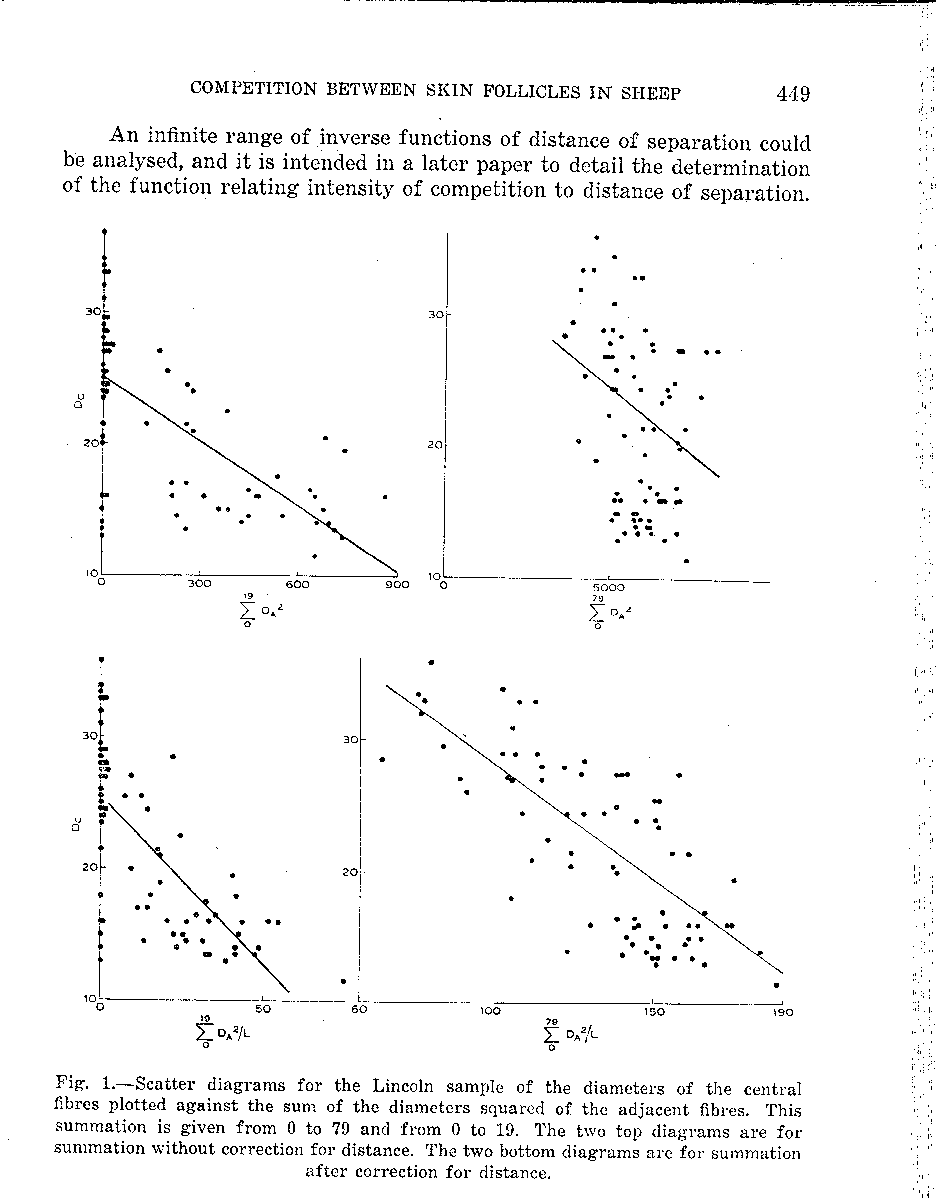
\includegraphics[width=1.0\textwidth]{frasershort.png}
%  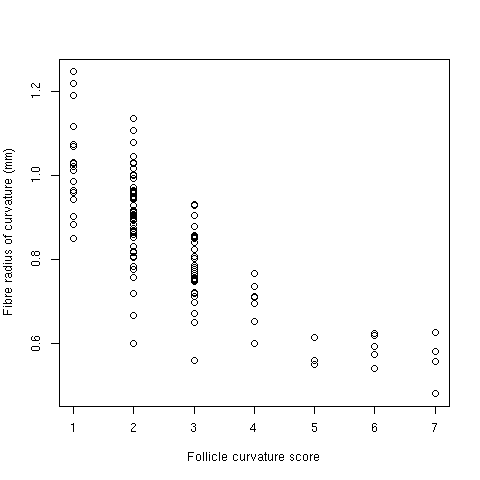
\includegraphics{ofdamm.png}
  \caption{Figure 1 from Fraser and Short(1952)~\cite{fras:52}. These data are for the Lincoln sheep only. The left side graphs are for the 147 micron circle, the right graphs for the 173 micron circle. The lower graphs are weighted by distance between follicles, the upper graphs are not weighted. }
  \label{fig:frasershort}
\end{figure}

%\end{document}


There is substantial variation around the regression line. This is not unexpected. Biological data are always noisy. This is the 'best' result - the Lincoln sample had the most significant regressions. We comment on this below. The weighting by distance did make some improvement.  The regressions were better for the smaller diameter circle. That all makes sense.

What we now have to do is delineate our areas of concern. These are as follows
\begin{description}
\item[follicle positions] these data came from horizontal sections of skin at sebaceous gland level. What is sectioned at that level is the follicle shaft, not the bulb.  Bulbs deviate substantially from the position of the shaft, especially in sheep with high follicle curvature. This is why the Lincoln data have a better fit - the positional information reflects the bulb position more accurately in the Lincoln because they have straight follicles. The Ryland and Merino specimens would have some degree of follicle curvature. 
It is the position of the bulb which may matter in relation to competition, because the bulb is the active tissue involved in growing fibre. 
\item[length growth rate] as a measure of fibre growth activity of the surrounding circle of skin, Fraser and Short used the sum of the squares of the diameters of all the follicles in the circle. This accounts for number of follicles, and fibre cross sectional area, but not fibre length growth rate.  We do not know if diameter and length are correlated in this scenario. So one part of their measure of follicle output of fibre is missing.
\item[confounding fibre growth and development] we are going to take a punt and assert that most of the regression significance comes from follicle number, rather than from diameter. Follicle number is purely a development factor. It does not change as the follicles grow fibre in the adult. So the contribution of follicle number to the regression is not at all an indicator of competition between fibres while they are growing fibre. It may indicate competition during development, but more recent work (Moore etal (1998)~\cite{moor:98}) indicates that it reflects variation in numbers of sites occupied by papilla cells, or, in the case of Merion sheep, follicles formed by branching from other follicles. 

Diameter, on the other hand, could reflect either factors operating during development ( such as the number of papilla cells that aggregate at sites) or factors that operate during fibre growth ( such as the expansion and shrinkage of follicles that occurs over the hair growth cycle, or with nutritional and photoperiodic variations). So diameter mixes up developmental factors with adult growth factors.  We suggest that the diameter effect on the regressions is likely to have been minimal - ie it is all about follicle number, which means it is all about development, not current growth.
\end{description}

Is there any way we can address these issues. Yes. The paper says
\begin{quote}
"The data from which the analysis detailed below was made are very bulky and have been lodged, with the accompanying statistical condensations and copes of the original drawings, with CSIRO Head Office Library, Melbourne, where they can be consulted. "
\end{quote}
Maybe we should request access to these data, and see if we can redo the analyses separately for follicle number and fibre diameter. That would at least address the third point above.

\subsection{Follicle groups}
One of the messages from the classic papers of H.B. Carter (Carter(1943)~\cite{cart:43} and Carter and Hardy (1947)~\cite{cart:47}) is that the {\em trio group} of three primary follicles and numbers of associated secondary follicles is the {\em biological unit} of sheep skin. What happens inside one trio group is repeated all over the woolgrowing surface, with some variations according to body sites. Whan you switch to  a different sheep, you may get a slightly differnet trio group, but it is again repeated all over the body.

So it has to be said that a large part of variation in fibre diameter between fibres within a fleece is due to variations in follicle and skin structure within the trio group. So studying trio groups is an important approach to trying to understand what controls fibre diameter variation. 

Unfortunately data on trio groups, particularly with fibre diameters measured, is rather limited. 

\subsection{Where to ?}
The mere idea of unequal sharing of some resource among follicles does not help much sort out why the shares are unequal. That is what we need to know - who or what is dealing out the resource unequally, and on what basis.

One thing is certain. We need to get quantitative.  That is what the next section is about. We try to get some real data on length and diameter, and to write some equations.

\section{Fibre length growth rate and fibre diameter}
This is about quantifying individual fibre length growth rates and fibre diameters and trying to write some equations defining how length growth rate and diameter are related to each other and to other things. So we are putting explanations on hold and trying to establish some facts.

\subsection{Fibre growth equations}
\subsection{Data on length growth rate and diameter for individual fibres}
\subsection{Cell model for fibre growth}

\section{Discussion}




\begin{thebibliography}{99}

\bibitem{cart:43}
Carter, H.B. (1943) Studies in the Biology of the Skin and Fleece of Sheep. 1. The development and general histology of the follicle group in the skin of the Merino. 2. The use of the tanned sheepskin in the study of follicle population density. 3. Notes on the arrangement, nomenclature, and variation of skin folds in the Merino. CSIR Bulletin No 164, Melbourne, 1943

\bibitem{cart:47}
Carter, H.B. and Hardy, M.H. (1947) Studies in the Biology of the Skin and Fleece of Sheep. 4. The hair follicle group and its topographical variations in the skin of the Merino foetus. CSIR Bulletin No 215, Melbourne, 1947

\bibitem{fras:51}
Fraser, A.S. and Short, B.F. (1951) Competition between skin follicles in sheep. Nature 167:202-203

\bibitem{fras:52}
Fraser, A.S. and Short, B.F. (1952) Competition between skin follicles in sheep Aust. J. agric. Res. 3(4):445-452

\bibitem{fras:53}
Fraser, A.S.(1953) Factors in the genetic determination of fleece structure in sheep. J. Genet. 51:222-236

\bibitem{fras:60}
Fraser, A.S. and Short, B.F. (1960) The Biology of the Fleece. Animal Research Laboratories Technical Paper No 3. CSIRO, Australia, 1960

\bibitem{hori:53}
Horio, M. and Kondo, T. (1953) Text. Res. J. 23:373

\bibitem{jack:16}
Jackson, N. and Watts, J.E. (2016) Staple crimp formation in the fleece of Merino sheep. Unpublished manuscript, 18 May 2016.


\bibitem{jack:18}
Jackson, N. and Moore, G.P.M. (2018)
Dynamics of pre-papilla cell numbers in sheep foetus and effect on follicle development URL https://github.com/nevillejackson/Fleece-biology/tree/master/pre-papilla-cells/ppcell.pdf

\bibitem{moor:84}
Moore G.P.M. and Jackson, N. (1984) An hypothesis implicating a founder cell pop
ulation in the regulation of wool follicle formation and distribution in sheep s
kin. J. Embryol. Exp. Morph. 82 (Suppl), 259

\bibitem{moor:89}
Moore G.P.M., Jackson, N., and Lax, J. (1989) Evidence of a unique developmental mechanism specifying both wool follicle density and fibre size in sheep selected for single skin and fleece characters. Genet. Res. Camb. 53:57-62

\bibitem{moor:98}
Moore, G.P.M., Jackson, N., Isaacs, K., and Brown, G (1998) J. Theoretical Biology 191:87-94

\bibitem{nay:66}
Nay T. (1966) Wool follicle arrangement and vascular pattern in the Australian Merino. Aust. J. agric. Res. 17:797-805

\bibitem{nayj:73}
Nay, T. and Jackson, N. (1973) Effect of changes in nutritional level on the depth and curvature of wool follicles in Australian Merino sheep. Aust. J. Agric. Res. 24:439-447

\bibitem{onio:62}
Onions, W.J. (1962) Wool: an introduction to its properties, varieties, uses
     and production. Ernest Benn limited, London, 1962

\bibitem{rprog:13}
R Core Team (2013). R: A language and environment for statistical
  computing. R Foundation for Statistical Computing, Vienna, Austria.
  ISBN 3-900051-07-0, URL http://www.R-project.org/.

\bibitem{ryde:55}
Ryder, M.L. (1955) The blood supply to the wool follicle. Proc. Int. Wool Textile Res. Conf. Aust. 1955. Volume F. pp63-90

\bibitem{swan:93}
Swan, P.G. (1993) Objective measurement of fibre crimp curvature and the bulk compressional properties of Australian wools. PhD Thesis, University of NSW, March 1993 

\bibitem{swan:99}
Swan, P.G. (1999) An explanation of the genetics of wool fibre diameter. Unpublished manuscript.

\end{thebibliography}
\end{document}
